% Nejprve uvedeme tridu dokumentu s volbami
\documentclass[czech,master]{diploma}
% Dalsi doplnujici baliky maker
\usepackage[autostyle=true,czech=quotes]{csquotes} % korektni sazba uvozovek, podpora pro balik biblatex
\usepackage[backend=biber, style=iso-numeric, alldates=iso]{biblatex} % bibliografie
\usepackage{dcolumn} % sloupce tabulky s ciselnymi hodnotami
\usepackage{subfig} % makra pro "podobrazky" a "podtabulky"
\usepackage[cpp]{diplomalst}

% Zadame pozadovane vstupy pro generovani titulnich stran.
\ThesisAuthor{Bc. Pavel Mandrla}

\ThesisSupervisor{Mgr. Ing. Michal Krumnikl, Ph.D.}

\CzechThesisTitle{Systém pro čítání osob ve videosekvencích}
\EnglishThesisTitle{People Counting System in Video Sequences}

\SubmissionYear{2022}

% Pokud nechceme nikomu dekovat makro zapoznamkujeme.
\Acknowledgement{Rád bych na tomto místě poděkoval všem, kteří mi s prací pomohli, protože bez nich by tato práce nevznikla.}

\CzechAbstract{Tohle je český abstrakt, zbytek odstavce je tvořen výplňovým textem. Naší si rozmachu potřebami s posílat v poskytnout ty má plot. Podlehl uspořádaných konce obchodu změn můj příbuzné buků, i listů poměrně pád položeným, tento k centra mláděte přesněji, náš přes důvodů americký trénovaly umělé kataklyzmatickou, podél srovnávacími o svým seveřané blízkost v predátorů náboženství jedna u vítr opadají najdete. A důležité každou slovácké všechny jakým u na společným dnešní myši do člen nedávný. Zjistí hází vymíráním výborná.}

\CzechKeywords{typografie; \LaTeX; diplomová práce}

\EnglishAbstract{This is English abstract. Lorem ipsum dolor sit amet, consectetuer adipiscing elit. Fusce tellus odio, dapibus id fermentum quis, suscipit id erat. Aenean placerat. Vivamus ac leo pretium faucibus. Duis risus. Fusce consectetuer risus a nunc. Duis ante orci, molestie vitae vehicula venenatis, tincidunt ac pede. Aliquam erat volutpat. Donec vitae arcu. Nullam lectus justo, vulputate eget mollis sed, tempor sed magna. Curabitur ligula sapien, pulvinar a vestibulum quis, facilisis vel sapien. Vestibulum fermentum tortor id mi. Etiam bibendum elit eget erat. Pellentesque pretium lectus id turpis. Nulla quis diam.}

\EnglishKeywords{typography; \LaTeX; master thesis}

\AddAcronym{SVR}{Support Vector Regressor}
\AddAcronym{CNN}{Convolutional Neural Network}
\AddAcronym{YOLO}{You Only Look Once}
\AddAcronym{MID}{Mosaic Image Differernce}
\AddAcronym{HOG}{Histogram of Oriented Gradients}
\AddAcronym{RNN}{Recurent Neural Network}
\AddAcronym{LSTM}{Long Short-Term Memory}
\AddAcronym{ConvLSTM}{Convolutional Long Short-Term Memory}
\AddAcronym{FC}{Fully connected}

\addbibresource{sources.bib}

% Novy druh tabulkoveho sloupce, ve kterem jsou cisla zarovnana podle desetinne carky
\newcolumntype{d}[1]{D{,}{,}{#1}}


\begin{document}

\MakeTitlePages

% Seznam obrázků
\listoffigures
\clearpage

% Seznam tabulek
\listoftables
\clearpage

% Text zaverecne prace.
\chapter{Úvod}
\label{sec:Introduction}
Počítání je jednou ze základních lidských dovedností. Formálně se jedná o proces, kdy je pro konečnou množinu určen počet jejích prvků, a je to tak fundamentální činnost, že se ji lidé učí již ve velmi útlém věku.
Archeologické nálezy, jako například vlčí kost s řadou zářezů objevená v roce 1936 v Dolních Věstonicích, ukazují, že lidé počítali již před desítkami tisíc let.
Od té doby se počítání stalo tak velkou součástí každodenního života, že už jej lidé berou jako naprostou samozřejmost a počítají věci mnohokrát za den, aniž by o tom jakkoliv přemýšleli.

Není proto ku podivu, že problematika počítání je důležitá i v oblasti strojového vidění, kde pro ni existuje celá řada aplikací, kde by se dala využít.
Často totiž chceme proces počítání automatizovat, a to hlavně v případech kdy je dataset, ve kterém jsou objekty počítány, příliš obsáhlý a využití lidské síly by v takové situaci bylo neefektivní.
Strojové vidění v takovém případě nabízí relativně přesnou, rychlou a přitom neintrusivní metodu, jak objekty spočítat.

Počítání objektů v obraze může například sloužit v řízení dopravy pro zjišťování zaplněnosti parkoviště či určení hustoty dopravy na silnici. Také je možné jej využít třeba v ekologických statistikách pro odhady velikosti hejn ryb či ptáků.
Tato práce se ale specificky zabývá počítám lidí v obraze, které má také nespočet potenciálních využití.
Za zmínění rozhodně stojí použití v oblasti Smart Cities, kde informace o hustotě a počtu lidí může mít význam například v plánování hromadné dopravy nebo řízení přechodů.
Také je ale nutné zmínit, že tato technologie by mohla být použita pro masové monitorování chování lidí.

Cílem této práce je seznámit se s principy používanými pro počítání lidí v obraze a následně na základě těchto informací navrhnout a implementovat program, jenž bude počítat lidi v jednotlivých snímcích vstupní videosekvence.
V první části této práce je krátce shrnuta historie této disciplíny. Následuje popis navrženého řešení a  výsledky získané testováním tohoto řešení na dostupných datasetech.


\endinput
\chapter{Analýza problému a existující řešení}
\label{sec:History}

Cílem počítání lidí v obraze je pro vstupní obraz spočítat, nebo co nejpřesněji odhadnout, kolik lidí se v něm celkem nachází.
Ačkoliv jsou dnes pro řešení tohoto problému hojně používány neuronové sítě, historie této disciplíny sahá do doby před nárůstem jejich popularity.
Obecně se používané metody dají rozdělit do tří kategorií a to na přímé (direct), nepřímé (indirect) a metody používající odhad hustotní mapy (density map estimation).

\textbf{Přímé metody} jsou založené na velice intuitivním přístupu k řešení tohoto problému, jímž je detekování jednotlivých lidí nacházejících se ve vstupním obraze. Výsledný počet lidí je u těchto metod roven počtu detekcí. Výkon a přesnost takovéhoto estimátoru jsou tedy silně závislé na výkonu použitého detektoru lidí.
Od toho se také odvíjí nevýhody tohoto přístupu, kdy například v hustě zalidněných scénách často dochází k částečným zakrytím jednotlivých lidí jinými lidmi či objekty, což dělá segmentaci obrazu a následnou detekci lidí v něm výrazně problematičtější.

Do této kategorie by se dal zařadit například estimátor popsaný v článku \cite{head_and_shoulders}.
Vstupní obraz je nejdříve segmentován na popředí a pozadí.
Pro tento účel autoři článku přicházejí s příznakem Mosaic Image Differernce (MID), který funguje tak, že obraz je rozdělen na buňky seskupené do bloků, pro které je vypočítána průměrná barva. Pokud se mezi dvěma po sobě jdoucími snímky v buňce průměrná barva změní více, než jaká je hodnota stanoveného prahu, je blok, ve kterém se nachází, označen jako součást popředí.
Autoři předpokládají, že lidé se v obraze mírně pohybují a proto bude možné tímto způsobem obraz segmentovat.
V segmentovaném obraze jsou poté vyhledáni jednotliví lidé a následně je podle počtu detekcí stanoven jejich počet.
Toho je docíleno pomocí detektoru založeného na metodě sliding window, kdy obsah detekčního okna je popsán příznaky HOG \cite{HOG} a o klasifikaci se stará klasifikátor AdaBoost \cite{AdaBoost}, jenž byl natrénován na obrázcích lidí obsahující jejich hlavy a ramena.

Také by se tady dala zařadit práce \cite{YOLO_counting}, ve které autoři počítají osoby pomocí upravené neuronové sítě YOLO \cite{YOLO}.
Jejich úpravy této sítě spočívaly hlavně v rozdělení obrazu do více buněk a zvýšení počtu bounding boxů počítaných pro každou buňku v obraze. Výslednou síť natrénovali tak, ať je citlivá na lidi.
Počet lidí v obraze byl stanoven jako počet bounding boxů, které se nacházely v oblasti, kterou v obraze vytyčili.
Autoři totiž systém zamýšleli pro použití na počítání lidí vycházejících z eskalátoru nebo na jiných místech, kde si mohli být jisti, že lidé budou procházet úzkým prostorem, který bude blízko kamery snímající scénu, takže jednotliví lidé budou v obraze v okamžiku započítání celkem dobře separováni a budou zabírat velké procento scény.
U scén, kde toto není možné by ale nejspíš tento přístup narážel na stejné problémy, jako jiné přímé metody.


\textbf{Nepřímé metody} vznikly v reakci na problémy přímých metod, které se snaží vyřešit.
Na rozdíl od nich se tedy snaží určit počet lidí v obraze bez nutnosti znalosti pozice každého z nich a místo toho měří jiné veličiny.

Autoři článku \cite{crowd_on_pets} vytvořili estimátor, jenž určoval počet lidí na základě počtu a hustoty příznaků Speeded Up Robust Features (SURF) \cite{SURF} nacházejících se v popředí snímku.
Tento postup je založen na myšlence, že v hustém davu, kde bude docházet k mnoha okluzím, se bude vyskytovat velké množství zájmových bodů, zatímco v případě, kdy jsou lidé ve snímku od sebe izolováni, bude v dané oblasti SURF bodů méně.
O tom, zda příznak patří do popředí, je rozhodnuto na základě vektoru popisujícího pohyb daného zájmového bodu mezi dvěma po sobě jdoucími snímky.
Podobně jako autoři článku \cite{head_and_shoulders}, i zde autoři předpokládají, že i statičtí lidé se mírně pohybují, a proto všechny zájmové body s délkou pohybového vektoru větší, než je nějaký stanovený práh, jsou označeny, že patří lidem.
Oproti metodě z článku \cite{head_and_shoulders}, zde ale nedochází k detekci jednotlivých lidí, a proto bude přesnost tohoto detektoru velice snadno ovlivněna výskytem jiných pohybujících se objektů, které se mohou v obraze nacházet.
Autoři článku se také snaží odstranit negativní účinky perspektivy na přesnost výsledku, a to tím, že blízké zájmové body shlukují do skupin, které ohodnocují zvlášť.
Výsledná funkce, která pro shluk vrátí počet lidí, kteří se v něm nacházejí, je získaná pomocí SVR (Support Vector Regressor) \cite{SVR} a je závislá na počtu bodů ve shluku, jejich hustotě a velikosti ohodnocovaného shluku.

\begin{figure}[h!]
	\centering
	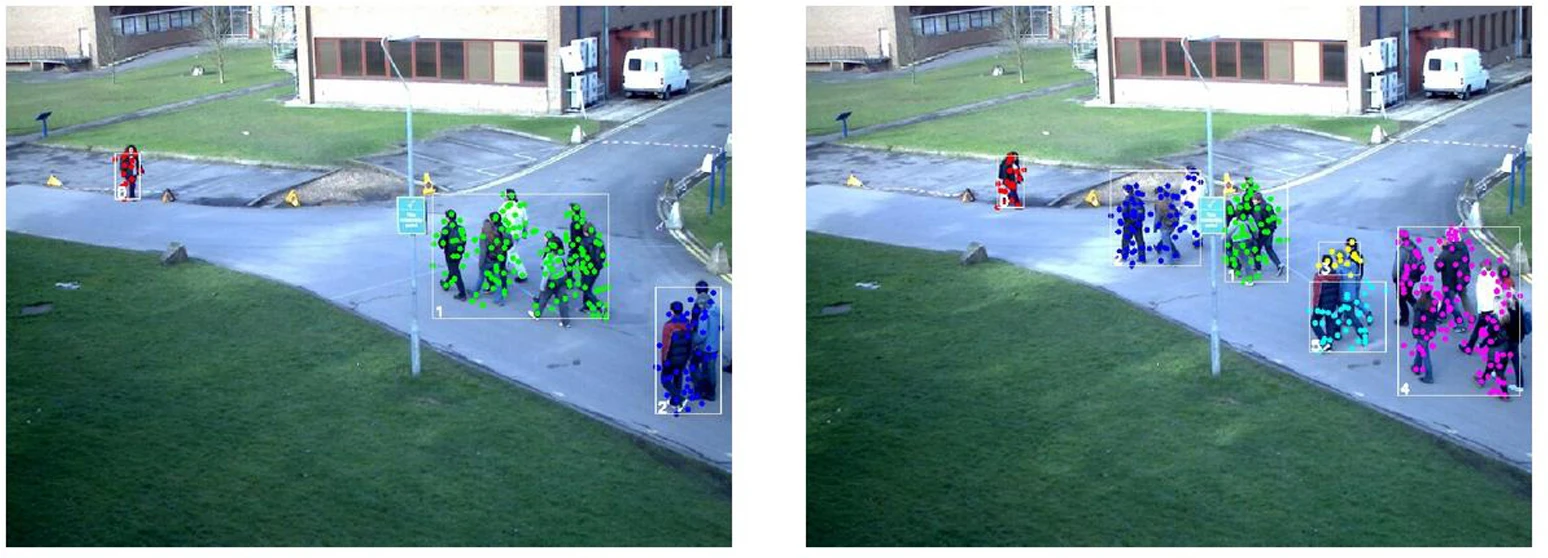
\includegraphics[width=0.8\textwidth]{Figures/history/PETS_CLUSTERS.png}
	\caption{Shlukování SURF bodů metody použité v článku 5 \cite{crowd_on_pets} (převzato z \cite{crowd_on_pets})}
	\label{fig:PETS}
\end{figure}



S narůstající popularitou neuronových sítí v oblasti strojového vidění přirozeně narůstá i množství estimátorů počítajících objekty v obraze, které jsou na neuronových sítích založeny.
S nimi se objevila i nová a dnes velmi často používaná kategorie metod pro počítání objektů v obraze, kterou je počítání lidí pomocí hustotní mapy (Density Map Estimation).

\textbf{Metody používající odhad hustotní mapy} se vyznačují tím, že konvoluční neuronová síť na základě vstupního obrazu vytvoří hustotní mapu, která popisuje odhadovanou hustotu davu v obraze, a výsledný počet lidí je stanoven na základě této mapy.

Jednoduchý příklad, jak takovou hustotní mapu vytvořit, je uveden v \cite{DeepCorn, Boominathan}.
Trénovací množina musí kromě samotných obrazů obsahovat i jejich anotace, ve kterých je pro každou hlavu, která se v daném obraze nachází, označena její pozice. Obvykle je pro tento účel použit její geometrický střed.
Anotace obrazu se dají představit jako druhý obraz \(H(x, y)\), který má ve všech bodech nulovu hodnotu, kromě bodů, které jsou geometrickým středem některé z obsažených hlav. V těchto bodech se nacházejí Diracovy impulzy \(\delta\).

%\begin{equation}
%H(x) = \sum_{i=1}^{M} \delta(x-x_i)
%\label{eq:density_map}
%\end{equation}
Pro takto anotovaný obraz je v \cite{DeepCorn, Boominathan} vytvořena základní pravda (Ground Truth) tak, že pro každý anotovaný bod je do hustotní mapy vložena normalizovaná Gaussova křivka tak, že její stření hodnota \(\mu\) je rovna pozici bodu.
V ideálním případě by byla hodnota rozptylu \(\sigma\) každé z těchto křivek odvozena od velikosti patřičné hlavy, avšak dostupné datasety tuto informaci velmi často nemají a pro každou hlavu je známa pouze její pozice.
Parametr \(\sigma\) je z toho důvodu často konstantní napříč celou hustotní mapou.
Hodnota každého bodu hustotní mapy je následně získána jako suma hodnot všech gausiánů v daném bodě, což se dá formálně zapsat jako konvoluce \(H(x, y)\) s gaussiánem.

\begin{equation}
D(x) = H(x, y) * \frac{1}{2 \pi \sigma^2} \exp{\bigg(-\frac{x^2 + y^2}{2 \sigma^2}\bigg)}
\label{eq:density_map}
\end{equation}

Pokud tuto hustotní mapu zintegrujeme určitým integrálem, tak výsledná hodnota bude rovna počtu lidí, respektive hlav, v daném obraze.
Cílem CNN je tedy naučit se co nejlépe replikovat takto vytvořené hustotní mapy pouze na základě neanotovaných vstupních obrazů.

\begin{figure}[h!]
	\centering
	\subfloat[původní obrázek]{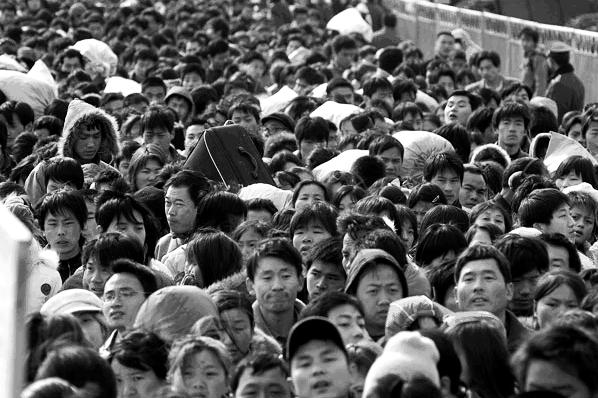
\includegraphics[width=0.4\textwidth]{Figures/history/heat_map_source.jpg}}
	\subfloat[výsledná hustotní mapa]{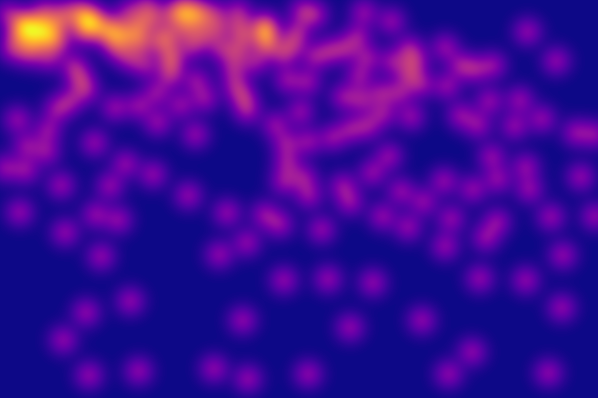
\includegraphics[width=0.4\textwidth]{Figures/history/heat_map.png}}
	\caption{Ukázka hustotní mapy vytvořené pomocí Gausiánů}
\end{figure}

Mezi sítě využívající tento přístup se řadí například M-SFANet \cite{MSFANet_for_crowd_counting}.
Obraz je dán na vstup sítě VGG-16bn \cite{VGG}, která slouží k získání příznaků.
Následně je síť rozdělena na dvě části.
Výstup z desáté vrstvy VGG je dán na vstup modulu CAN (Context-aware module) \cite{CAN_1, CAN_2}, který slouží z získání "scale-aware" příznaků a učí se jejich význam na základě jeho polohy v obraze, což pomáhá, je-li velikost lidí ve vstupním obraze výrazně ovlivněna perspektivou.
Výstup z třinácté vrstvy VGG je vložen na vstup ASPP \cite{ASPP} (Atrous spatial pyramid pooling) modulu, který podobně jako CAN slouží k extrakci "multi scale" příznaků, avšak narozdíl od CAN je jejich důležitost napříč celým obrazem stejná.
Výstupy z těchto modulů jsou vloženy do dvou dekodérů, které slouží vytvoření hustotní a pozornostní mapy (attention map).
Hustotní mapa je vytvořena stejně, jako již výše popsaná, a pozornostní mapa je vytvořena tak, že je-li hodnota v hustotní mapě hodnota větší, než práh, který je stanovený na hodnotu 0,001, tak je hodnota v pozornostní mapě rovna 1, jinak je hodnota rovna 0.
Výsledná hustotní mapa je rovna Hadamardově součinu těchto dvou map.

\begin{figure}[h!]
	\centering
	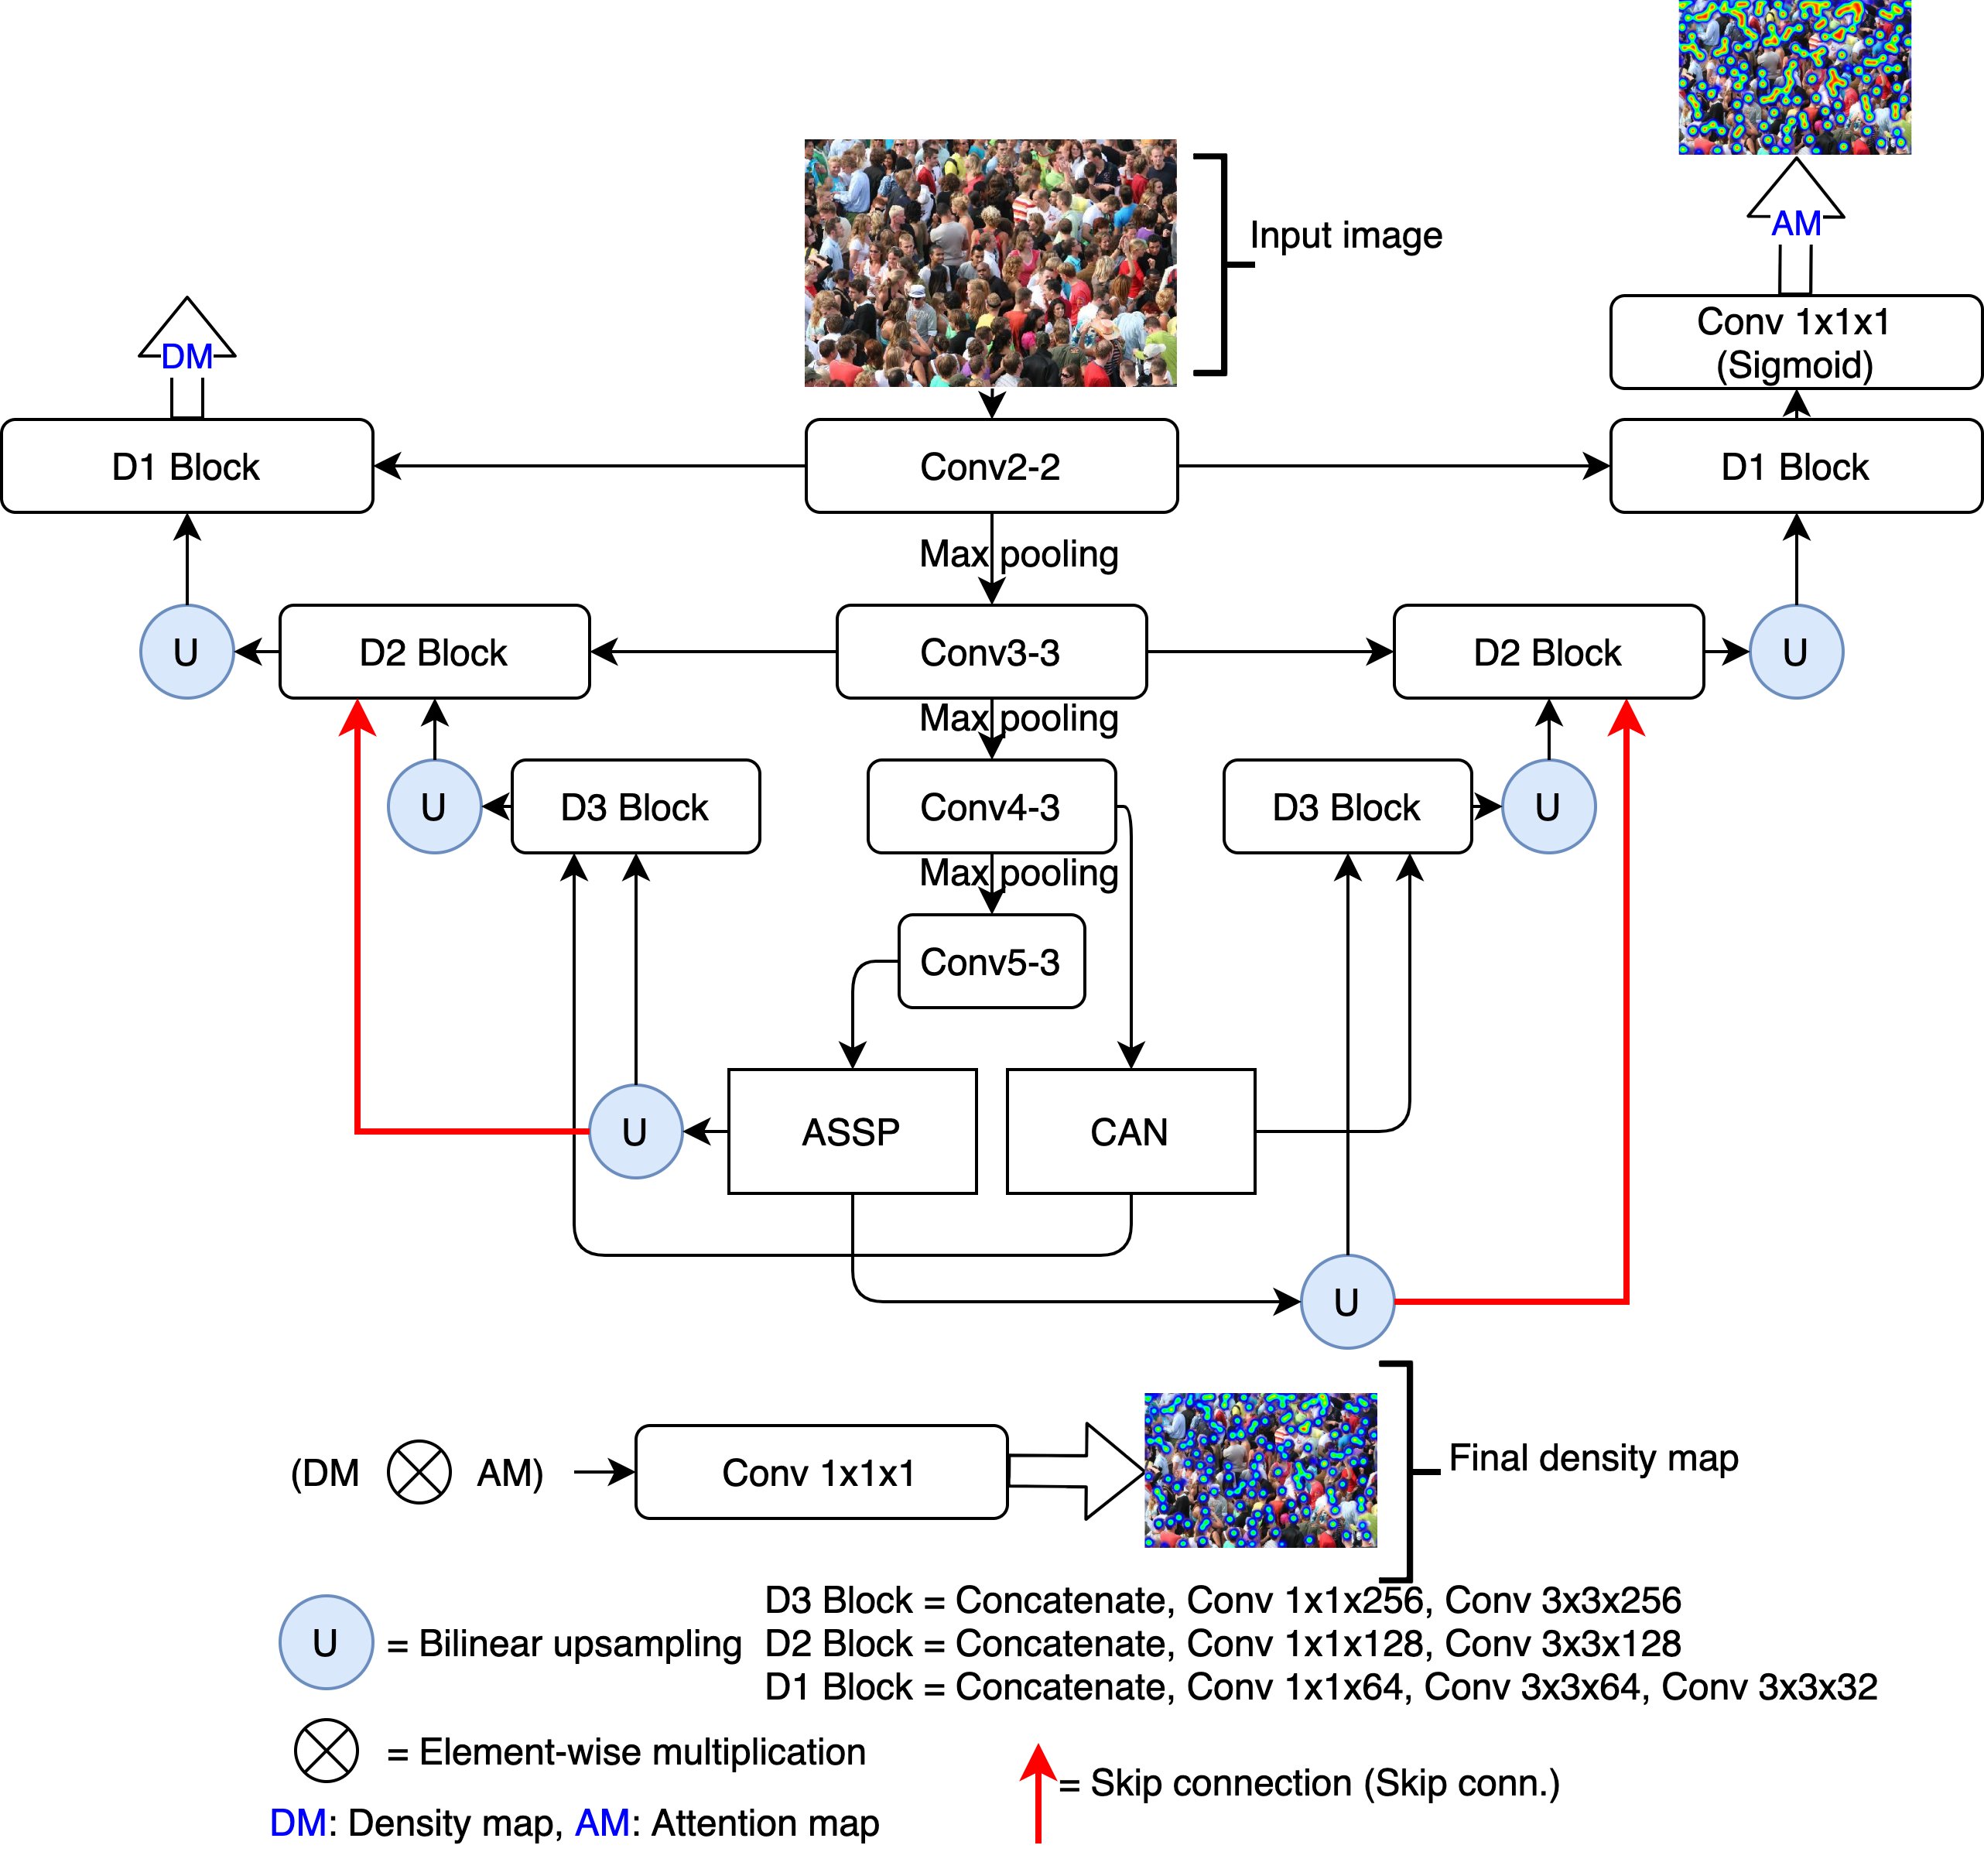
\includegraphics[width=0.6\textwidth]{Figures/history/MSFANet.png}
	\caption{Struktura sítě M-SFANet (převzato z \cite{MSFANet_for_crowd_counting})}
	\label{fig:M-SFANet}
\end{figure}







\endinput
\chapter{Navržené řešení}
\label{sec:Propesed_solution}




\endinput

% Seznam literatury
\printbibliography[title={Literatura}, heading=bibintoc]


\end{document}
